% Terminal records and all Observe answers.
\section{Environment}

All experiments were performed on 23 October 2026 inside \textbf{Ubuntu 26.04.1 LTS (ARM64)} running in VirtualBox as user \texttt{misa} on \texttt{UbuntuVM}. The Linux kernel is \texttt{7.0.0-38-generic}. The installed xv6 checkout is \texttt{\textasciitilde{}/\allowbreak{}xv6-riscv}, commit \texttt{06aad25c\allowbreak{}735fd315\allowbreak{}9bdfae56\allowbreak{}80be4eab\allowbreak{}7b1668b2}. GCC and the RISC-V compiler are version 15.2.0; QEMU is version 10.2.1. xv6 is booted from this Ubuntu with \texttt{make qemu CPUS=1}.

The figures are screenshots of the Ubuntu terminal during execution. Complete command output is provided in \texttt{terminal-output.txt}; build logs are in \texttt{build-output.txt} for the xv6 labs. PIDs, inode numbers and free-space values below refer to these recorded runs.

The xv6 image was rebuilt for this laboratory. Its Makefile retains the earlier lab utilities and adds run, runls, runmissing, pingpong and primes.

\begin{figure}[H]
\centering
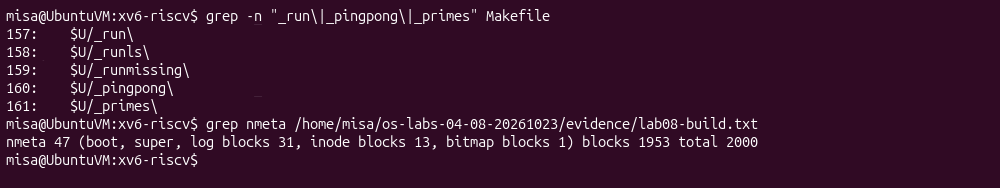
\includegraphics[width=\textwidth,height=0.74\textheight,keepaspectratio]{img/08_01_build.png}
\caption{The required programs are registered in UPROGS and the xv6 image builds inside Ubuntu.}
\end{figure}

\section{Part 1 - run inside xv6}

\texttt{user/\allowbreak{}run.c} follows the provided program. The parent prints its PID and forks; the child prints its own PID and calls exec with a NUL-terminated argument vector for echo. The parent waits for the child and prints the returned status. The ls variant is \texttt{user/\allowbreak{}runls.c}; the failed-exec variant is \texttt{user/\allowbreak{}runmissing.c}, leaving run as the default echo example.

\begin{figure}[H]
\centering
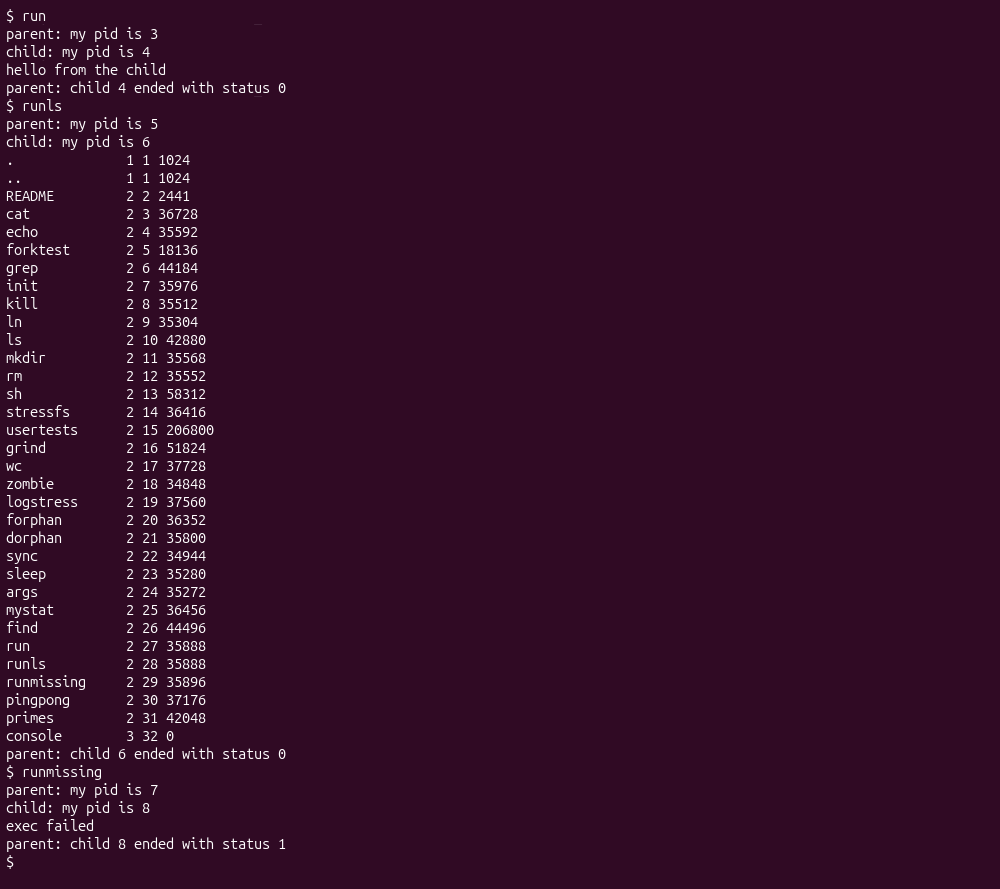
\includegraphics[width=\textwidth,height=0.74\textheight,keepaspectratio]{img/08_02_run.png}
\caption{Echo, ls and failed-exec variants executed in the xv6 booted from Ubuntu.}
\end{figure}

The first run used parent PID \textbf{3} and child PID \textbf{4}, printed \texttt{hello from the child}, and reported status 0. runls used PIDs 5/6, displayed the xv6 root listing and also reported 0. The nonexistent executable used PIDs 7/8, printed \texttt{exec failed} and reported status 1.

\subsection{1. Compare the three calls with Linux}

\begin{table}[H]\centering{\small\setlength{\tabcolsep}{4pt}\renewcommand{\arraystretch}{1.25}
\begin{tabular}{@{}>{\raggedright\arraybackslash}p{0.25\textwidth}>{\raggedright\arraybackslash}p{0.29\textwidth}>{\raggedright\arraybackslash}p{0.38\textwidth}@{}}
\toprule

\textbf{Operation} & \textbf{xv6 lab 08} & \textbf{Linux lab 07} \\ \midrule

Create the child & \texttt{fork()} & \texttt{fork()} \\

Replace its image & \texttt{exec("echo",\allowbreak{} args)} & \texttt{execlp("ls",\allowbreak{} "ls",\allowbreak{} "-l",\allowbreak{} (char *)NULL)} \\

Reap it & \texttt{wait(\&status)} & \texttt{waitpid(pid,\allowbreak{} \&status,\allowbreak{} 0)} \\

\bottomrule\end{tabular}}\end{table}

The process lifecycle is the same: fork creates a child with inherited memory contents and descriptors; exec replaces its program while retaining its PID; wait collects its termination information and reaps it. Linux execlp is a libc helper with PATH search and variadic arguments. xv6 exec takes a pathname and an argument vector directly, without PATH search. xv6 wait stores the exit value directly, whereas Linux waitpid returns an encoded status requiring wait macros.

\subsection{2. Who prints hello from the child?}

The echo executable prints it. run prints the PID messages before exec; successful exec never returns to that old image. echo receives the words in its argument vector and writes the resulting message.

\subsection{3. Why failure is 1 here and 127 on Linux}

The xv6 branch explicitly calls \texttt{exit(1)} after exec fails, while the Linux branch explicitly calls \texttt{exit(127)}. The programs choose those numbers; exec returns an error rather than automatically assigning an exit code. The xv6 parent still exits 0 after reporting the child, following the supplied example.

\section{Part 2 - pingpong}

\texttt{user/\allowbreak{}pingpong.c} creates parent-to-child and child-to-parent pipes and forks. Each process closes the ends it does not use. The parent sends one initialized byte; the child reads it, prints ping, sends the same byte back and exits. The parent reads the reply, prints pong, closes the remaining ends and reaps the child. Failures from pipe, fork, read, write and wait are checked.

\begin{lstlisting}[style=terminal]
parent p2c[1] -- one byte --> p2c[0] child
parent c2p[0] <-- one byte -- c2p[1] child
\end{lstlisting}

\begin{figure}[H]
\centering
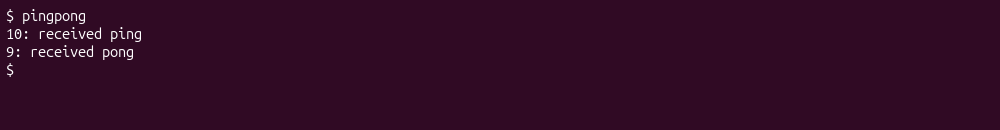
\includegraphics[width=\textwidth,height=0.74\textheight,keepaspectratio]{img/08_03_pingpong.png}
\caption{The child prints received ping before its parent prints received pong.}
\end{figure}

The child PID was \textbf{10} and the parent PID was \textbf{9}. The child prints ping before writing the reply, and the parent prints pong only after receiving that byte. This data dependency guarantees the message order even if scheduling changes the timing.

\subsection{1. Why two pipes rather than one}

A pipe is a one-way byte stream with no addressed messages. A separate pipe for each direction gives each process a distinct input and output channel. If both processes read and write the same pipe, either could consume its own byte instead of the intended peer receiving it.

\subsection{2. Which call makes the parent wait for the reply}

\texttt{read(c2p[0],\allowbreak{} \&b,\allowbreak{} 1)} blocks until the child supplies a byte while a writer remains open. The later wait call reaps the child; it is not what synchronizes reception of the reply. Closing unused writers also makes EOF possible when the peer exits without replying.

\section{Optional - Primes}

\texttt{user/\allowbreak{}primes.c} generates integers 2 through 35 and creates a chain of filtering processes. Each filter reads its first number as a prime, prints it, and forwards only numbers not divisible by it to the next stage. Each process closes its unused pipe ends and its output end when input reaches EOF, then waits for its child.

\begin{figure}[H]
\centering
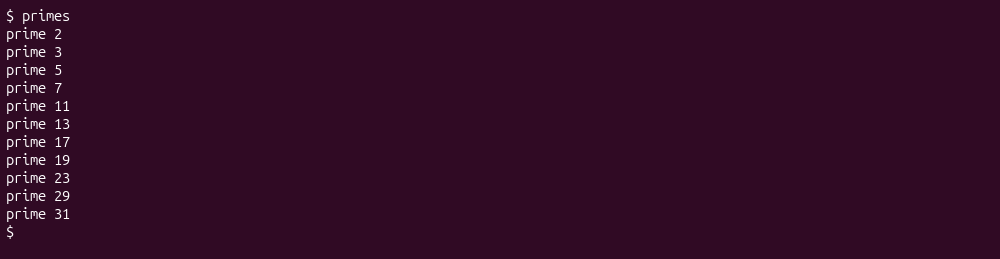
\includegraphics[width=\textwidth,height=0.74\textheight,keepaspectratio]{img/08_04_primes.png}
\caption{The process-chain sieve prints every prime from 2 through 35 and terminates.}
\end{figure}

The actual output is \textbf{2, 3, 5, 7, 11, 13, 17, 19, 23, 29, 31}, exactly the eleven primes in that inclusive interval. Closing the final writers propagates EOF through the chain and lets every filter exit. Retaining only necessary descriptors also respects xv6's per-process descriptor limit.
